%%%%%%%%%%%%%%%%%%%%%%%%%%%%%%%%%%%%%%%%%%%%%%%%%%%%%%%%%%%%%%%%%%
\begin{figure}[t!]
\centerline{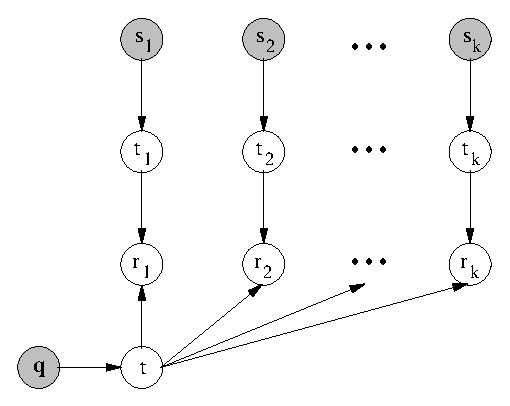
\includegraphics[scale = .8]{graphicalModel}}
\vspace{-2mm}
\caption{Latent subtopic binary relevance model.}
\vspace{-3mm}
\label{fig:gm}
\end{figure}
%%%%%%%%%%%%%%%%%%%%%%%%%%%%%%%%%%%%%%%%%%%%%%%%%%%%%%%%%%%%%%%%%%
We propose a directed graphical model in Figure~\ref{fig:gm} to formalize the independence assumptions in a probabilistic subtopic model of binary relevance. In Figure~\ref{fig:gm}, shaded nodes represent observed variables, whereas unshaded nodes are latent. The observed variables are the query terms $\vec{q}$ and selected items $s_i$ (where for $1 \leq i \leq k$, $s_i\in D$).  For the subtopic variables, let $T$ be a discrete subtopic set.  Then $t_i \in T$ represent subtopics for respective
$s_i$ and $t \in T$ represents a subtopic for query $\vec{q}$.  The
$r_i$ are binary variables that indicate if respective selected
items $s_i$ are relevant ($r_i=1$).

The conditional probability tables (CPTs) are as follows: $P(t_i|s_i)$
and $P(t|\vec{q})$ respectively represent the subtopic distribution
for item $s_i$ and query $\vec{q}$.  The remaining CPTs are 
for the relevance variables $r_i$, using $\I[\cdot]$ as a $\{0,1\}$ indicator function (1 if $\cdot$ is true), item $s_i$ is deemed \emph{relevant} \emph{iff} \emph{its subtopic $t_i$ matches query subtopic $t$}:
\begin{align*}
P(r_{i}=1|t, t_{i}) & \; = \; \I[t_{i} = t]
\end{align*}
Here, $\I[\cdot]$ is $1$ when its argument is true and $0$ otherwise.

Given the specification of the graphical model, now we formally define two objectives \emph{expected 1-call@$k$} and \emph{expected n-call@$k$}. The \emph{expected 1-call@$k$} objective is defined below: 
\begin{align}
\label{eq:setRelevance}
    \ExpOneCall(S_k,\vec{q}) & = \mathbb{E} \left[\left. \bigvee_{i=1}^{k}r_i=1 \right| s_{1},\dots, s_{k},\vec{q} \right], 
\end{align}

In order to define the expected \emph{expected n-call@$k$}, we denoted by $R_k = \sum_{i=1}^k r_i$, where $R_k$ is 
the number of relevant items from the first $k$ selections.  
Reading $R_k \geq n$ as $\I[R_k \geq n]$, we express the \emph{expected $n$-call@$k$} objective as 
\begin{align}
\label{eq:setRelevance}
  \ExpNCall{n}(S_k,\vec{q})
  = \mathbb{E}[R_k\geq n|s_1,\dots,s_k,\vec{q}] .  
\end{align}
Since jointly optimizing either $\ExpOneCall(S_k,\vec{q})$ or $\ExpNCall{n}(S_k,\vec{q})$ is NP-hard, we
take a greedy approach similar to MMR where we choose the best $s_k^*$
assuming that $S_{k-1}^*$ is given, and present the main derivaiton results in the following section. 
